%!TEX root = ../../main.tex
\section{PSU}
\begin{figure}[H]
	\centering
	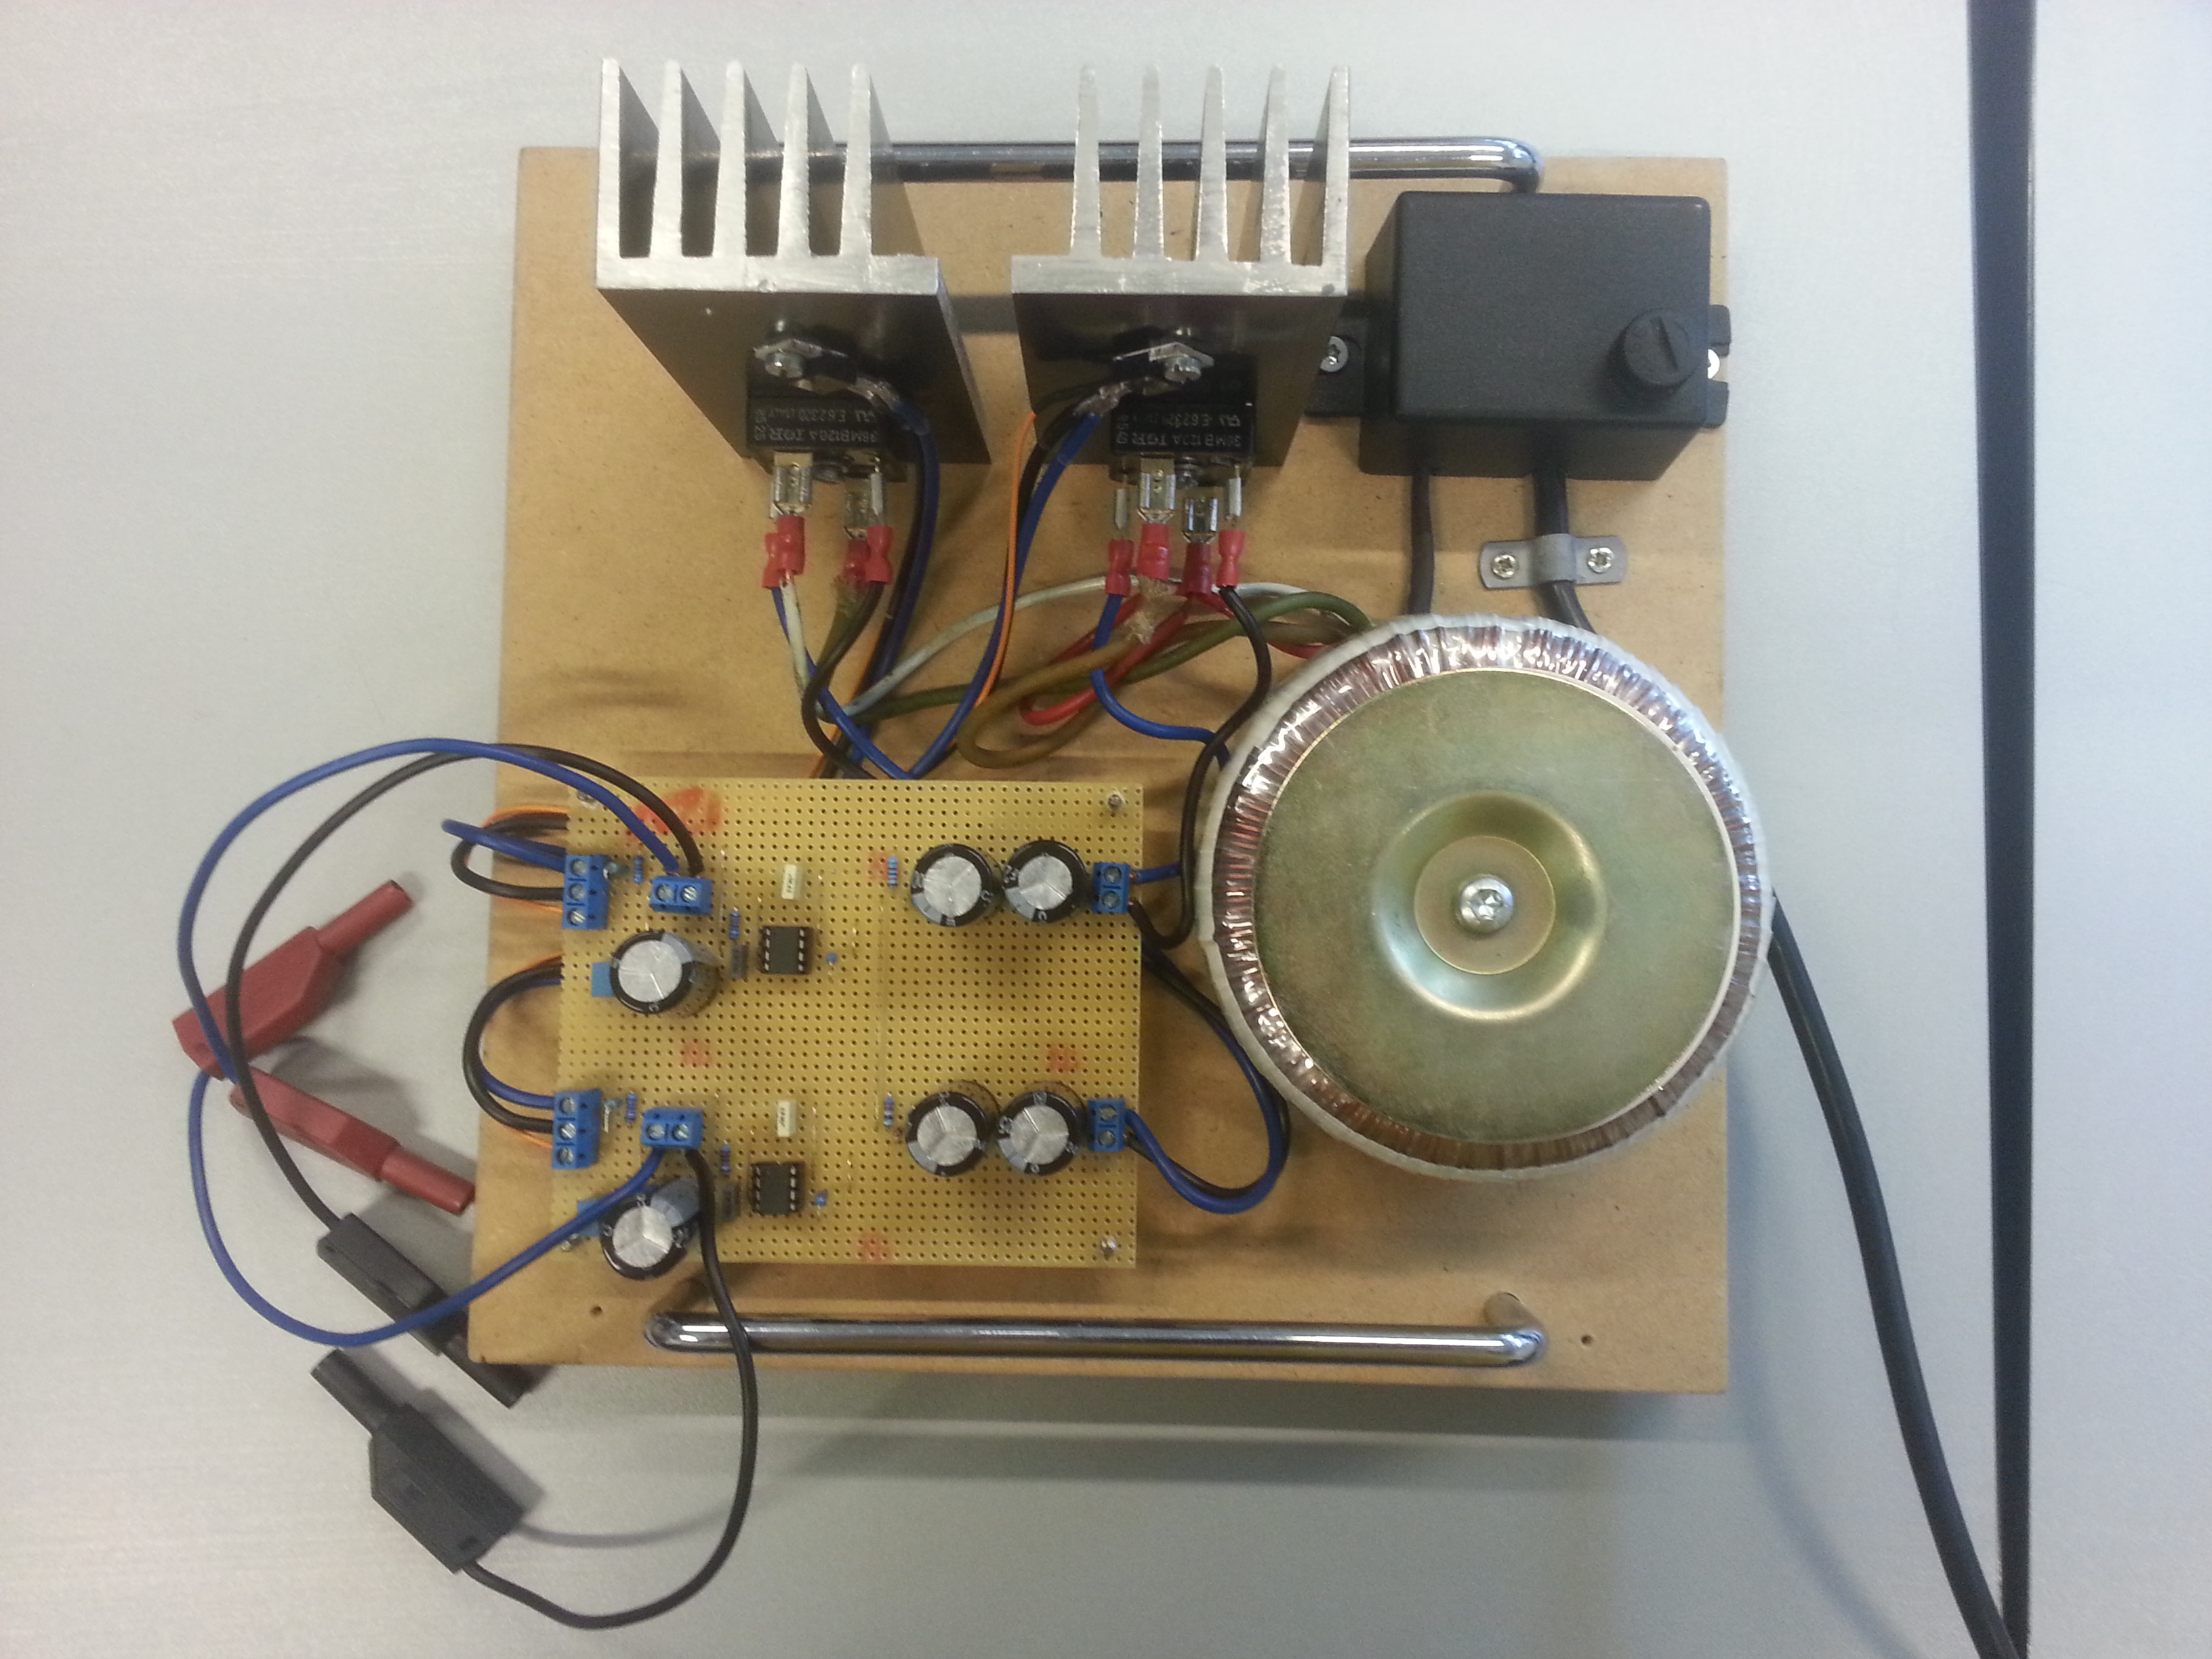
\includegraphics[scale=0.1]{../Hardware/PSU/PSU}
	\caption{Strømforsyningen}
	\label{photo:PSU}
\end{figure}

\subsection{Analyse}
For at få en idé om det maksimale forbrug, vil der blive kigget på den absolut maksimale strøm for hver del. Der forekommer følgende behov for systemet (12VDC):
\begin{itemize}
\item Pumpen PWM styres ved 12VDC. Ved 100\% positiv duty cycle vil den trække 3A.
\item Ventilerne forsynes med 12VDC. De vil hver især maksimalt trække 0,5A pr. styk.
\end{itemize}

Nu er det værd at kigge på, hvornår den største belastning af strømforsyningen forekommer. Ud fra de specificerede
usecases, er den maksimale belastning 1 pumpe og 1 ventil på samme tid. Dette sker f.eks. ved "Manuel Vanding". Ved et større system med flere
sensor-øer vil kravet selvfølgelig være større.
\\\\
Resten af systemet er forsynet med 5VDC. Der er følgende behov:
\begin{itemize}
\item Central Control. Består af en Raspberry Pi 2. Fra databladet udledes, at den trækker imellem 0,6-2,5A. Grunden til det store strømforbrug er,
at der sidder 4 USB-stik på som hver kan trække op til 500mA. Da vi ikke udnytter dette, kan der regnes med maksimalt 0,6A.
\item Flowmåler. Bruger ca. 15mA. Tages ikke med i udregningen grundet det lille forbrug.
\item Kar- og Ø-controller. Består af en PSoC som normaltvis forsynes via. USB, altså maksimalt 0,5A pr. styk. Prototypen består af 3 PSoCs, derfor regnes der med 1,5A.
\item RSConverter. Forbruget er udregnet til 150mA. Prototypen består af 4, altså 0,6A.
\end{itemize}

Specifikationer for 12VDC- og 5VDC-forsyningen er nu givet. Et bud på et samlet forbrug vil være:
\begin{equation}
	I_{5V} = 0,6A + 1,5A + 0,6A = 2,7A
\end{equation}

\begin{equation}
	I_{12V} = 3A + 0,5A = 3,5A
\end{equation}

Kredsløbene er vist herunder:
\begin{figure}[H]
	\centering
	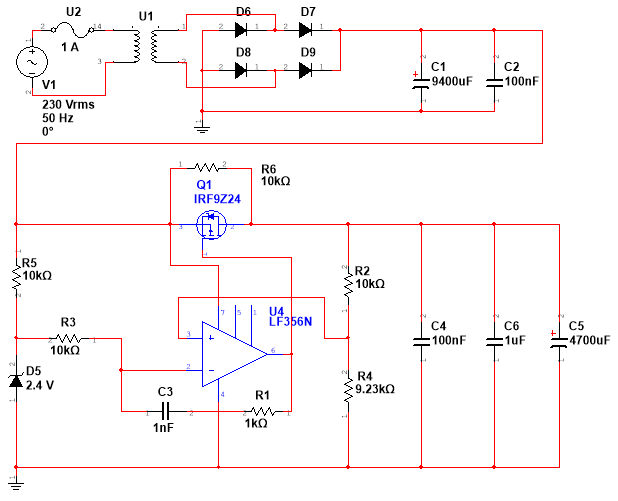
\includegraphics[scale=0.75]{../Hardware/PSU/PSU_5V}
	\caption{5V strømforsynings diagram}
	\label{photo:PSU_5V}
\end{figure}

\begin{figure}[H]
	\centering
	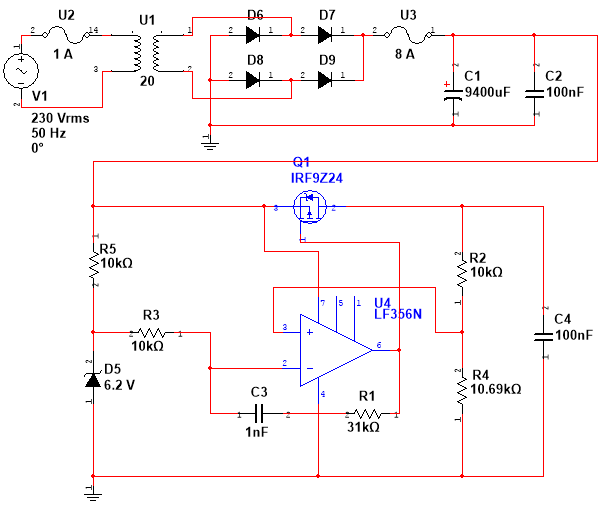
\includegraphics[scale=0.75]{../Hardware/PSU/PSU_12V}
	\caption{12V strømforsynings diagram}
	\label{photo:PSU_12V}
\end{figure}

Begge reguleringskredsløb opbygges efter samme princip. Fælles for de 2 er:
\begin{itemize}
\item 230VAC-1A sikring
\item 230VAC-2x12VAC transformer
\end{itemize}

Herefter består hvert kredsløb af:
\begin{itemize}
\item Diodebro: D6, D7, D8, D9
\item Kapacitet: C1, C5
\item Afkoblingskondensatorer: C2, C4, C6
\item Referencespænding: R5, D5
\item Fejlforstærker: U4, R1, R3, C3
\item Spændsføler på udgangen: R2, R4
\item FET til regulering: Q1
\item Opstartsmodstand: R6
\end{itemize}

Spændingen fra el-nettet transformeres fra 230VAC til 12VAC. Herefter dobbelt-ensrettes det:

\begin{figure}[H]
	\centering
	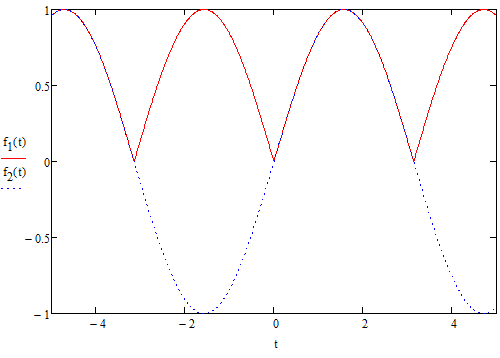
\includegraphics[scale=1]{../Hardware/PSU/Ensretning}
	\caption{Ensrettet spænding}
	\label{photo:Ensrettet}
\end{figure}

$f_1(t)$ er det ensrettede signal, hvor $f_2(t)$ er det oprindelige signal fra elnettet.
\\\\
Der vil derfor nu forekomme en 12VAC 100Hz spænding. Denne spænding lader C1 op og C1 vil derefter aflade når spændingen falder.
Dette glatter spændingen ud og resultat vil være tæt på et DC signal. Jo mere strøm der trækkes ud af denne kobling, jo mere kapacitet er der brug for.
AC-spændingen er regnet i RMS, derfor kræver det en lille omregning til peak-peak spænding og dermed VDC:
\\\\
\begin{equation}
	V_{DC} = V_{AC} * \sqrt{2} = 16,92V
\end{equation}
\\\\
Der vil nu ligge en stabil DC-spænding. Nu er spændingen ensrettet og udglattet. For at give 5VDC og 12VDC kræves det at spændingen reguleres.
For at kunne regulere spændingen, kræves et referencepunkt. Dette punkt er skabt ved R5 og D5. Zenerdioden sørger for en præcis spænding
i punktet, 6,2V eller 2,4V. Næste del er en fejlforstærker der kigger på udgangsspændingen i forhold til referencepunktet.
Til dette anvendes en operationsforstærker. Minus-indgangen forbindes igennem R3 til referencepunktet. Plus-indgangen forbindes til
spændingsdeleren som føler på udgangen. R1 og C3 bestemmer sammen med R3 forstærkningen. En ligning kan opstilles for forstærkningen:
\\\\
\begin{equation}
	A = 1 + \frac{R_1 + \frac{1}{2*\pi*f*C_3}}{R_3} = 1 + \frac{1k\ohm + \frac{1}{2*\pi*f*1nF}}{10k\ohm}
\end{equation}
\\\\
Ved at indføre C3 opnåes en frekvensafhængig forstærkning. Dette gøres for at undgå at højfrekvent støj kan forstyrre reguleringen.
For at give et eksempel af forstærkningen, udregnes der 5 eksempler med hhv. DC (0Hz), 1kHz, 10kHz, 100kHz og $f = \infty$.
Da forstærkningen i en operationsforstærker selvfølgelig ikke er uendelig, vil den være lig med $A_{OL}$ (se billedet fra databladet for LF356 herunder).

\begin{figure}[H]
	\centering
	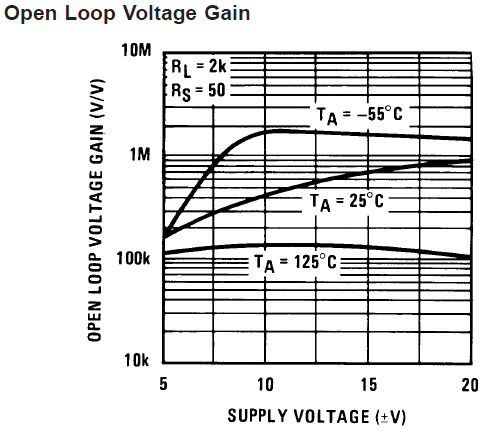
\includegraphics[scale=0.5]{../Hardware/PSU/OpenLoop}
	\caption{Open loop karakteristik for LF356}
	\label{photo:OpenLoop}
\end{figure}

\begin{equation}
	A_{OL} = 700 * 10^3
\end{equation}

\begin{equation}
	A_{DC} = 1 + \frac{1k\ohm + \frac{1}{2*\pi*0*1nF}}{10k\ohm} = A_{OL}
\end{equation}

\begin{equation}
	A_{1kHz} = 1 + \frac{1k\ohm + \frac{1}{2*\pi*1kHz*1nF}}{10k\ohm} = 17,015
\end{equation}

\begin{equation}
	A_{10kHz} = 1 + \frac{1k\ohm + \frac{1}{2*\pi*10kHz*1nF}}{10k\ohm} = 2,692
\end{equation}

\begin{equation}
	A_{100kHz} = 1 + \frac{1k\ohm + \frac{1}{2*\pi*100kHz*1nF}}{10k\ohm} = 1,259
\end{equation}

\begin{equation}
	A_{\infty} = 1 + \frac{1k\ohm + \frac{1}{2*\pi*\infty*1nF}}{10k\ohm} = 1,1
\end{equation}
\\\\
Udgangen af operationsforstærkeren styrer gaten på en P-kanal FET. I databladet for IRF9Z24 findes følgende oplysninger:
\begin{itemize}
\item $R_{DS(on)} = 0,28\ohm$ når $V_{GS} = -10V$
\item $I_D = -11A$ når $T = 25^{\circ}C$ og  $I_D = -7,7A$ når $T = 100^{\circ}C$
\item $P_D = 60W$
\end{itemize}

Den maksimale strøm der trækkes ved 12V er 3,5A og ved 5V er den 2,7A. Den afsatte effekt i FET'en kan dermed udregnes:
\\\\
\begin{equation}
	P_{5V} = (16,97V - 5V) * 2,7A = 32,321W
\end{equation}

\begin{equation}
	P_{12V} = (16,97V - 12V) * 3,5A = 17,397W
\end{equation}
\\\\
For at kunne klare denne effekt, skal de 2 FETs monteres på køleplader.

\begin{figure}[H]
	\centering
	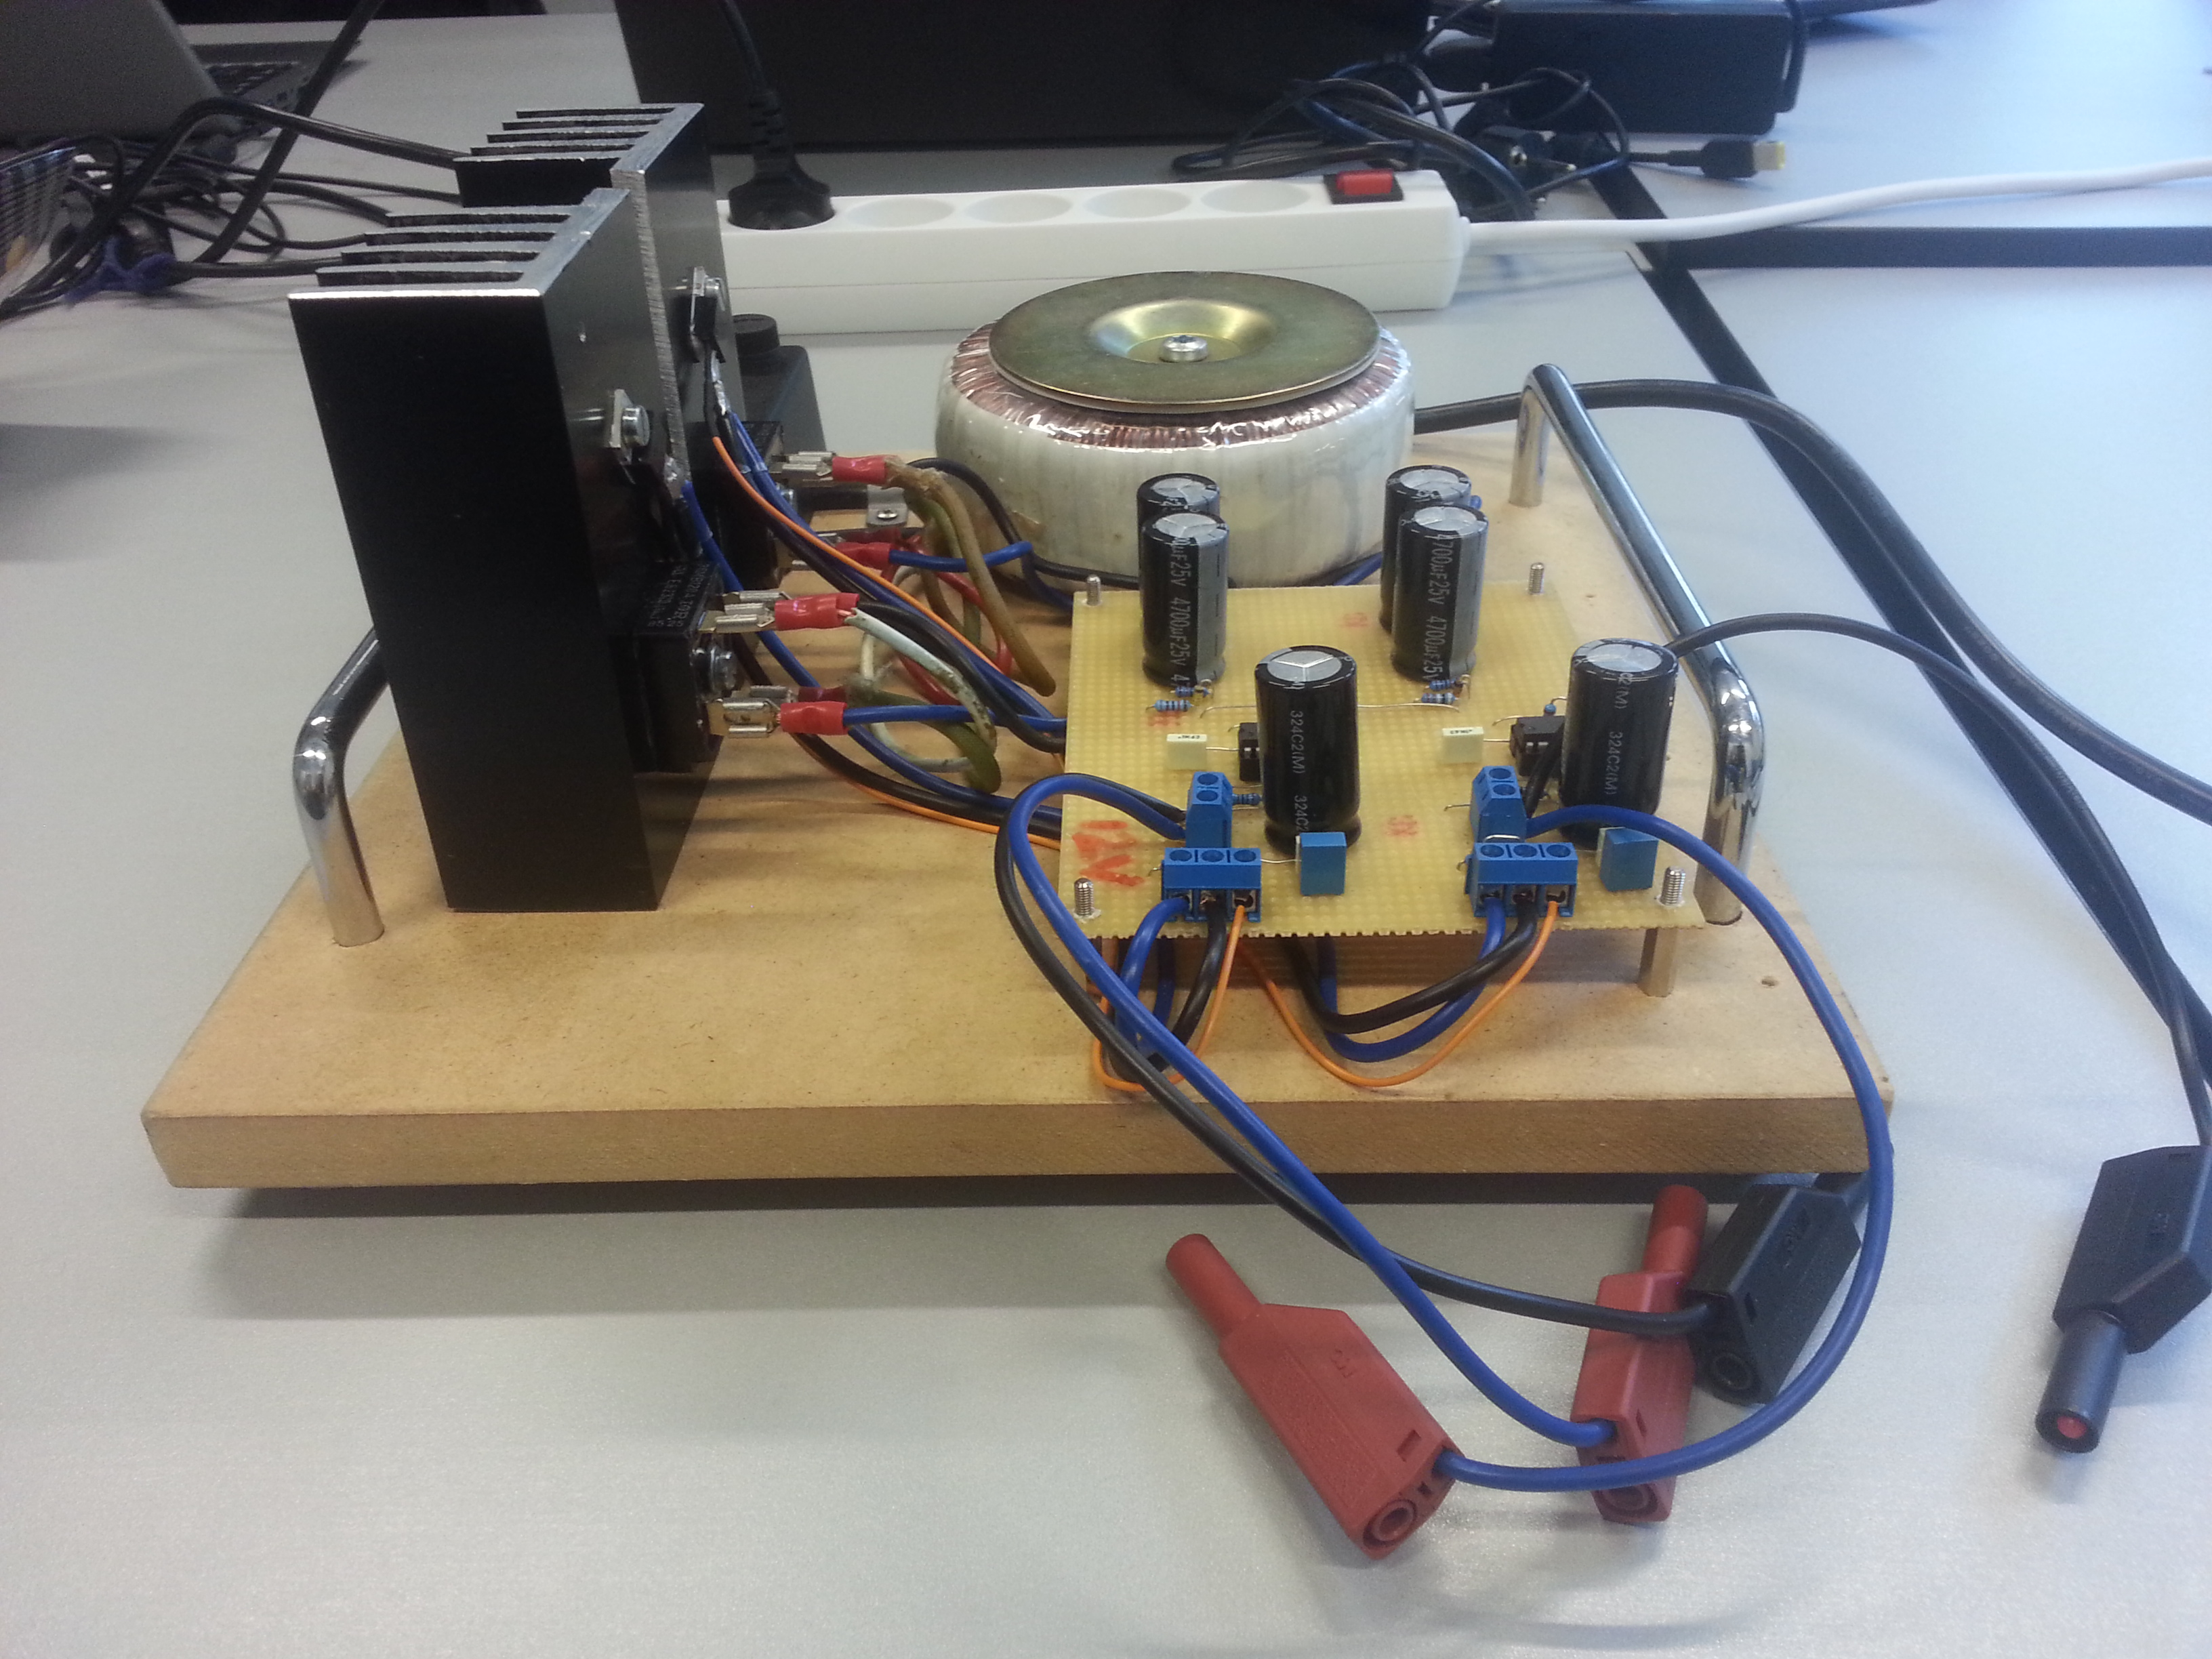
\includegraphics[scale=0.1]{../Hardware/PSU/Koeleplade}
	\caption{Strømforsyningens køleplader}
	\label{photo:Koeleplade}
\end{figure}

I tilfælde af at operationsforstærkeren lukker for FET'en inden den når at lade en spænding igennem, monteres der en opstartsmodstand henover FET'en (fra source til drain).
Denne sørger for at C5 lades op og spændingsføleren giver nu en spænding ind til fejlforstærkeren. Når denne spænding så overstiger referencepunktet,
vil fejlforstærkeren regulere det ved at hæve spændingen på FET'ens gate.


\subsection{Realisering}
Kredsløbet er opbygget på VERO board. Udgangen skal belastes med effektmodstande så de trækker de udregnede maksimal-værdier.
Størrelsen af effekt modstandene beregnes:
\begin{equation}
	R_{5V} = \frac{5V}{2,7A} = 1,852\ohm
\end{equation}

\begin{equation}
	R_{12V} = \frac{12V}{3,5A} = 3,429\ohm
\end{equation}

Til rådighed findes der følgende effektmodstande:
\begin{itemize}
\item 2 stk. $5\ohm$
\item 4 stk. $10\ohm$
\end{itemize}

Følgende opstillinger kommer tættes på den ønskede belastning:
\begin{equation}
	R_{5V_{realisering}} = (5^{-1} + 5^{-1} + 10^{-1} + 10^{-1})^{-1} = 1,667\ohm
\end{equation}

\begin{equation}
	R_{12V_{realisering}} = (10^{-1} + 10^{-1} + 10^{-1})^{-1} = 3,333\ohm
\end{equation}

Testen kan nu opstilles, og resultatet samt opstillingen ses herunder:
\begin{figure}[H]
	\centering
	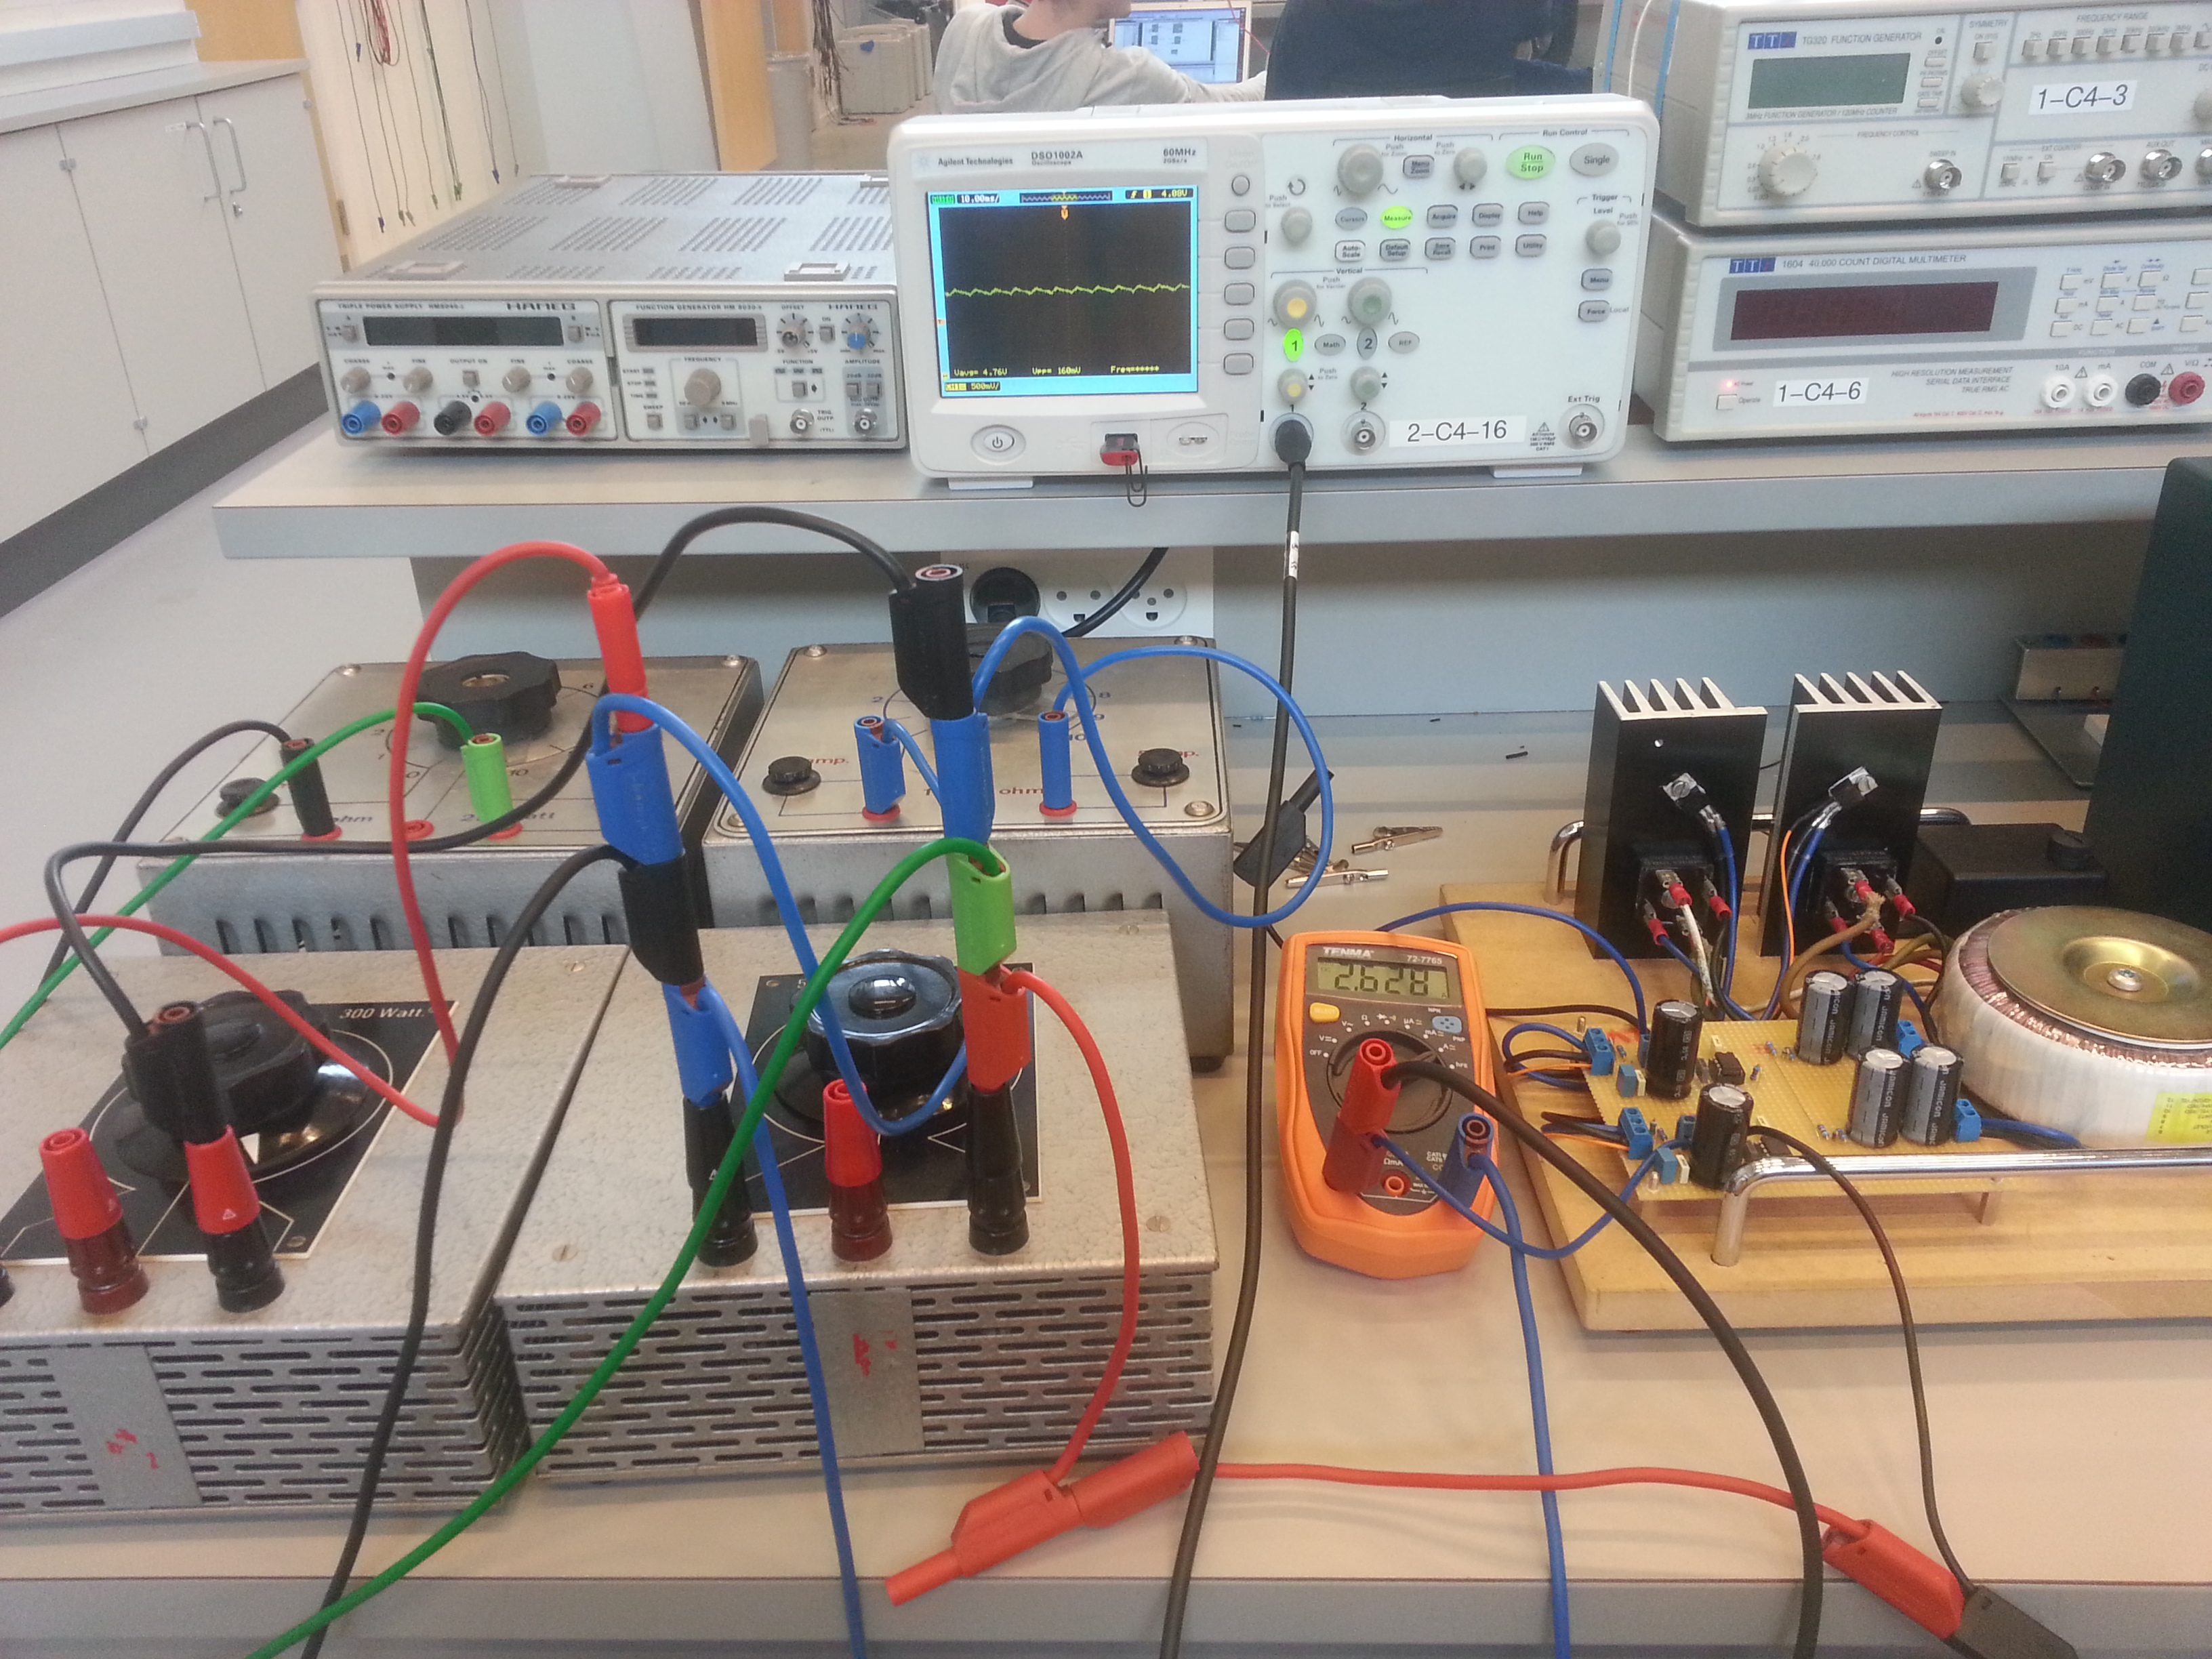
\includegraphics[scale=0.1]{../Hardware/PSU/Realisering/5VloadOpstilling}
	\caption{Testopstillingen med belastning på 5V forsyningen}
	\label{photo:5VloadOpstilling}
\end{figure}

\begin{figure}[H]
	\centering
	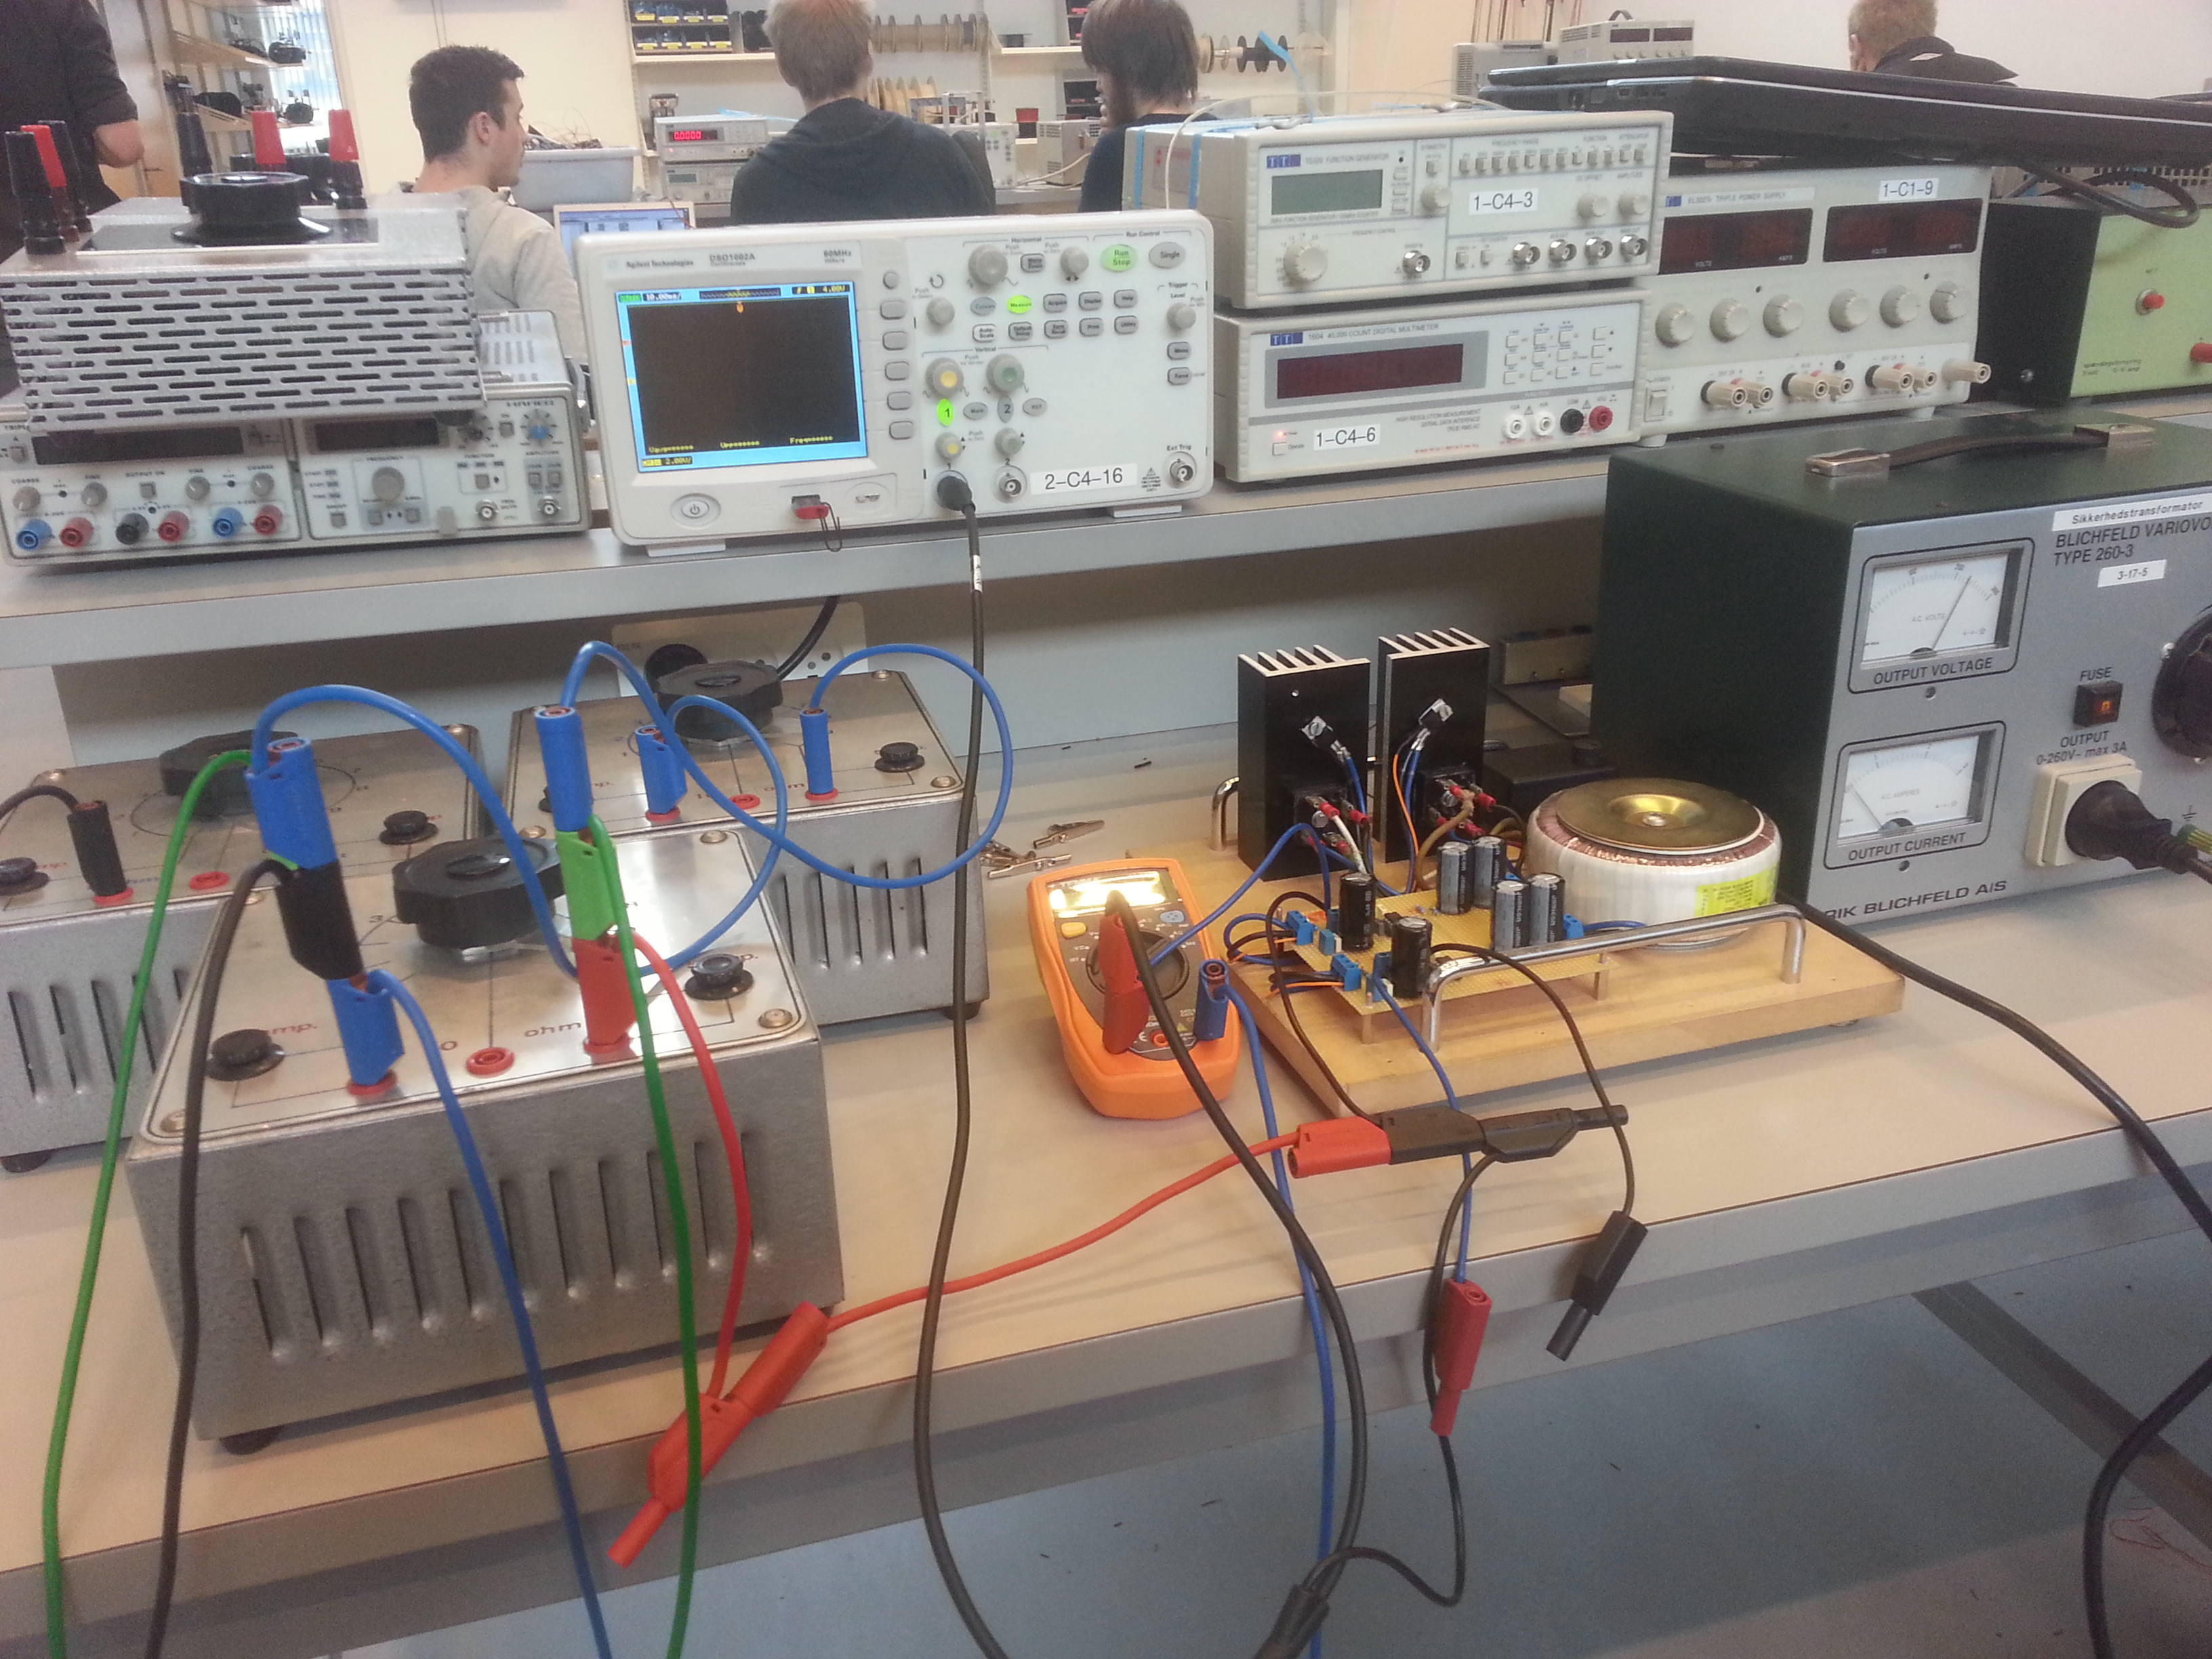
\includegraphics[scale=0.1]{../Hardware/PSU/Realisering/12VloadOpstilling}
	\caption{Testopstillingen med belastning på 12V forsyningen}
	\label{photo:12VloadOpstilling}
\end{figure}

\begin{figure}[H]
	\centering
	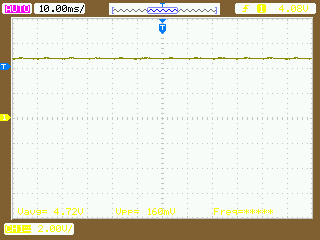
\includegraphics[scale=1]{../Hardware/PSU/Realisering/5VnoLoad}
	\caption{5V forsyningen uden belastning}
	\label{photo:5VnoLoad}
\end{figure}
\begin{figure}[H]
	\centering
	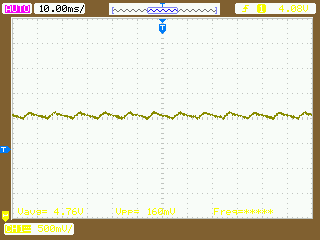
\includegraphics[scale=1]{../Hardware/PSU/Realisering/5VwithLoad}
	\caption{5V forsyningen med belastning}
	\label{photo:5VwithLoad}
\end{figure}
\begin{figure}[H]
	\centering
	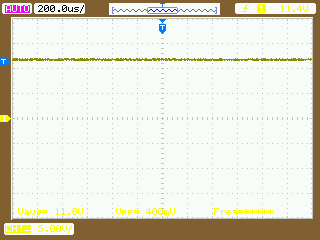
\includegraphics[scale=1]{../Hardware/PSU/Realisering/12VnoLoad}
	\caption{12V forsyningen uden belastning}
	\label{photo:12VnoLoad}
\end{figure}
\begin{figure}[H]
	\centering
	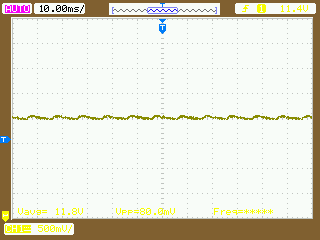
\includegraphics[scale=1]{../Hardware/PSU/Realisering/12VwithLoad}
	\caption{12V forsyningen med belastning}
	\label{photo:12VwithLoad}
\end{figure}

Som figur\ref{photo:5VwithLoad} viser, kommer der en rippel på forsyningen ved belastning. Rippelen på 5V-forsyningen giver følgende informationer:

\begin{itemize}
\item $V_{pp} = 160mV$
\item Periodetiden kan aflæses til $T = 10mS$ hvilket medfører en frekvens på $f = \frac{1}{T} = 100Hz$
\end{itemize}

100Hz frekvensen som optræder ved belastningen fortæller, at der er mangler på kapacitet. Når spændingen fra transformeren rammer dens peak-værdi, bliver kondensatoren $C_1$ ladet helt op. Men inden den næste peak-værdi forekommer, har kondensatoren afladet 160mV. Dette giver en rippel som kan fjernes ved at tilføre mere kapacitet.
\\\\
Samme fænomen ser vi, ved at kigge på figur\ref{photo:12VwithLoad}.
\begin{itemize}
\item $V_{pp} = 80mV$
\item Periodetiden kan aflæses til $T = 10mS$ hvilket medfører en frekvens på $f = \frac{1}{T} = 100Hz$ 
\end{itemize}

Det skal også noteres at begge forsyninger ikke rammer den ønskede spænding. Der er flere unøjagtigheder som kan påvirke dette:
\begin{itemize}
\item Unøjagtighed i zener-dioden $D_5$.
\item Offset i fejlforstærkeren $U_4$.
\end{itemize}


\subsubsection{Transformertest}
Transformeren tilfører et tab i strømforsyningen i form af følgende:
\begin{itemize}
\item Modstand i primær- og sekundær-vindinger
\item Leakage reaktans i primær- og sekundær-vindinger.
\item Jernkerne tab.
\item Magnetisk reaktans.
\end{itemize}


For at beregne disse faktorer foretages der 2 målinger:
\begin{itemize}
\item Short-circuit giver modstanden i vindingerne samt leakage reaktansen.
\item Open-circuit giver jernkernetabet og den magnetiske reaktans.
\end{itemize}


Short-circuit testen forbinder en variabel spændingskilde til primær-siden og kortslutter sekundær-siden.

\begin{figure}[H]
	\centering
	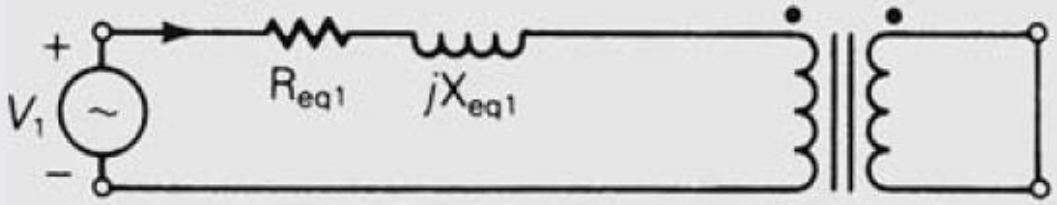
\includegraphics[scale=0.25]{../Hardware/PSU/Transformer/ShortCircuit}
	\caption{Short-circuit test}
	\label{photo:ShortCircuit}
\end{figure}

$R_{eq1}$ simulerer tabet i vindingerne. $X_{eq1}$ simulerer leakage reaktansen. Først findes den maksimale strøm som må løbe i primær-siden. Det udregnes således:

\begin{equation}
	I_{max} = \frac{S_{rated}}{V_{rated}} = \frac{160VA}{230V} = 0,696A
\end{equation} 


Spændingen på skille-varioen justeres fra 0VAC indtil strømmen er $I_{max} = 0,696A$. Spændingen aflæses til $V_{sc} = 18V$. Nu kan den aktive effekt beregnes:

\begin{equation}
	P_{sc} = V_{sc} * I_{max} = 18V * 0,7A = 12,522W
\end{equation}


Nu kan tabene beregnes:

\begin{equation}
	R_{eq1} = \frac{P_{sc}}{I_{max}^2} = \frac{12,522W}{(0,696A)^2} = 25,875\ohm
\end{equation}
\begin{equation}
	\left|Z_{eq1}\right| = \frac{V_{sc}}{I_{max}} = \frac{18V}{0,696A} = 25,875\ohm
\end{equation}
\begin{equation}
	X_{eq1} = \sqrt{\left(\left|Z_{eq1}\right|\right)^2 - R_{eq1}^2} = 0
\end{equation}
\begin{equation}
	Z_{eq1} = R_{eq1} + j * X_{eq1} = 25,875\ohm
\end{equation}


Open-circuit testen forbinder en 230V spændingskilde til primær-siden og sekundær-siden står ubelastet.

\begin{figure}[H]
	\centering
	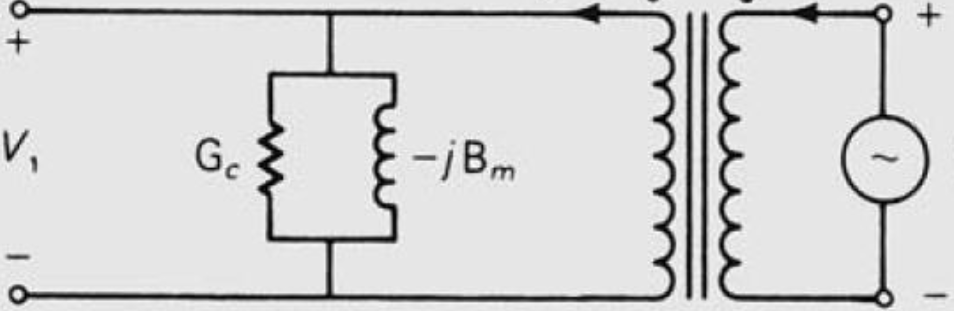
\includegraphics[scale=0.25]{../Hardware/PSU/Transformer/OpenCircuit}
	\caption{Open-circuit test}
	\label{photo:OpenCircuit}
\end{figure}


Spændingen på skille-varioen sættes til 230VAC. Tomgangsstrømmen skal aflæses og den aktive effekt beregnes:

\begin{equation}
	I_{oc} = 10mA
\end{equation}
\begin{equation}
	P_{oc} = V_{rated} * I_{oc} = 230V * 10mA = 2,3W
\end{equation}


Nu kan tabene beregnes:

\begin{equation}
	N_1 = 12
\end{equation}
\begin{equation}
	N_2 = 230
\end{equation}
\begin{equation}
	V_1 = \frac{N_1}{N_2} * V_{rated} = \frac{12}{230} * 230 = 12V
\end{equation}
\begin{equation}
	G_C = \frac{P_{oc}}{V_1^2} = \frac{2,3W}{12V^2} = 16mS
\end{equation}
\begin{equation}
	\left|Y_m\right| = \frac{\frac{N_2}{N_1} * I_{oc}}{V_1} = \frac{\frac{230}{12} * 10mA}{12V} = 16mS
\end{equation}
\begin{equation}
	B_m = \sqrt{\left|Y_m\right|^2 - G_C^2} = 0
\end{equation}
\begin{equation}
	Y_m = G_C = j * B_m = 16mS
\end{equation}


\subsubsection{Fremtidigt arbejde}
Der var umiddelbart 2 forbedringer som ville give en mere stabil og funktionel strømforsyning. Først og fremmest skal der indføres mere kapacitet på udgangen af strømforsyningen. Dette vil fjerne eller i hvert fald formindske den rippel som opstår ved større belastninger. For det andet kan der indføres et potmeter i spændingsføleren, som derved kan justere udgangsspændingen. Dette vil samtidig også gøre, at begge kredsløb (til 5V og 12V) kunne være ens. Det giver også mulighed for at lave andre spændinger ud fra kredsløbet.
\\\\
Til et færdigt produkt er der stadig meget arbejde med f.eks. at udligge print og konstruere et chassis som strømforsyningen og ikke mindst kølepladerne kan placeres i.